\documentclass{standalone}
\usepackage{tikz}
\begin{document}
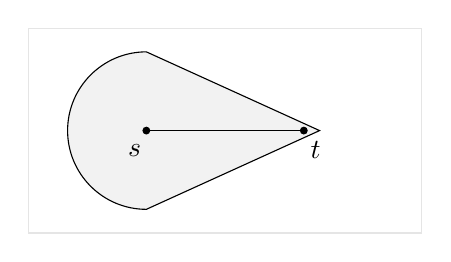
\begin{tikzpicture}

\filldraw[fill=black!5, draw=black]
   (3.7,0) -- (1.5,1) arc (90:270:1) -- cycle;
\fill[black] (1.5,0.0) circle (0.05);
\node at (1.35,-0.25) {$s$};
\fill[black] (3.5,0.0) circle (0.05);
\node at (3.65,-0.25) {$t$};
\draw (1.5,0.0) -- (3.5,0.0);

% border
\draw[black!10] (0.0,-1.3) rectangle (5.0,1.3);

\end{tikzpicture}%
\end{document}
